\documentclass[
]{jss}

%% recommended packages
\usepackage{orcidlink,thumbpdf,lmodern}

\usepackage[utf8]{inputenc}

\author{
James Hollway\\Graduate Institute of\\
International and Development Studies \And Henrique Sposito\\Graduate
Institute of\\
International and Development Studies
}
\title{Working with Unspecified, Approximate, Uncertain, Sets and Ranges
of Dates with \pkg{messydates}}

\Plainauthor{James Hollway, Henrique Sposito}
\Plaintitle{Working with Unspecified, Approximate, Uncertain, Sets and
Ranges of Dates with messydates}
\Shorttitle{\pkg{messydates}: An R package for ISO's Extended Date/Time
Format}


\Abstract{
This paper presents the \pkg{messydates} package for R, which
facilitates working with `messy' dates. Messy dates are dates that
include some imprecision and do not easily fit within the standard date
format because they are historical, ambiguous, approximate, unspecified
or uncertain, or otherwise admit of a range or set of possible dates.
Messy dates are common when studying historical but also potentially
current phenomena. Oftentimes, researchers will elect to pretend as if a
messy date is more precise than it is to make it compatible with other
more precise dates and to use various tools of temporal analysis such as
event history analysis. The paper highlights these problems and offers
practical advice on how to solve them using \pkg{messydates}. The paper
also introduces a conceptual framework for resolving messydates into
more familiar date classes in R ready for analysis.
}

\Keywords{dates, ISO, \proglang{R}}
\Plainkeywords{dates, ISO, R}

%% publication information
%% \Volume{50}
%% \Issue{9}
%% \Month{June}
%% \Year{2012}
%% \Submitdate{}
%% \Acceptdate{2012-06-04}

\Address{
    James Hollway\\
    Graduate Institute of\\
International and Development Studies\\
    Chemin Eugène-Rigot 2A\\
PO Box 1672\\
1211 Geneva 1\\
Switzerland\\
  E-mail: \email{james.hollway@graduateinstitute.ch}\\
  URL: \url{http://jameshollway.com}\\~\\
    }


% tightlist command for lists without linebreak
\providecommand{\tightlist}{%
  \setlength{\itemsep}{0pt}\setlength{\parskip}{0pt}}

% From pandoc table feature
\usepackage{longtable,booktabs,array}
\usepackage{calc} % for calculating minipage widths
% Correct order of tables after \paragraph or \subparagraph
\usepackage{etoolbox}
\makeatletter
\patchcmd\longtable{\par}{\if@noskipsec\mbox{}\fi\par}{}{}
\makeatother
% Allow footnotes in longtable head/foot
\IfFileExists{footnotehyper.sty}{\usepackage{footnotehyper}}{\usepackage{footnote}}
\makesavenoteenv{longtable}



\usepackage{amsmath}

\begin{document}



\hypertarget{introduction}{%
\section{Introduction}\label{introduction}}

Dates are often messy. Whether historical (or ancient), future, or even
recent, we sometimes only know approximately when an event occurred,
that it happened within a particular period, or sources offer multiple
competing dates. Messy dates are dates that include some degree of
imprecision.

\pkg{messydates} implements for R the Extended Date/Time Format (EDTF)
annotations set by the International Organization for Standardization
(ISO) outlined in \href{https://www.iso.org/standard/70908.html}{ISO
8601-2\_2019(E)}. The extended format allows for standardised annotation
of date imprecision so interpretation is unambiguous and
interoperability is guaranteed. These include notation for:

\begin{longtable}[]{@{}
  >{\centering\arraybackslash}p{(\columnwidth - 6\tabcolsep) * \real{0.2593}}
  >{\raggedright\arraybackslash}p{(\columnwidth - 6\tabcolsep) * \real{0.1358}}
  >{\raggedright\arraybackslash}p{(\columnwidth - 6\tabcolsep) * \real{0.1852}}
  >{\raggedright\arraybackslash}p{(\columnwidth - 6\tabcolsep) * \real{0.4198}}@{}}
\toprule()
\begin{minipage}[b]{\linewidth}\centering
Date type
\end{minipage} & \begin{minipage}[b]{\linewidth}\raggedright
Annotation
\end{minipage} & \begin{minipage}[b]{\linewidth}\raggedright
Example
\end{minipage} & \begin{minipage}[b]{\linewidth}\raggedright
Explanation
\end{minipage} \\
\midrule()
\endhead
unspecified date(component)s & \texttt{X} & \texttt{2012-XX-01} & The
first day of some unknown month \\
approximate date(component)s & \texttt{\textasciitilde{}} &
\texttt{2012-01-12\textasciitilde{}} & Approximately the 12th of January
2012 \\
uncertain date(component)s & \texttt{?} & \texttt{2012-01-12?} & The
data point is based on an unreliable source \\
sets of dates & \texttt{\{\}} & \texttt{\{2012-01-01,\ 2012-01-12\}} &
Date can be either 1 January 2012 and 12 January 2012 \\
ranges of dates & \texttt{..} & \texttt{2012-01-01..\ 2012-01-12} & All
dates between the 1 January 2012 and 12 January 2012 \\
\bottomrule()
\end{longtable}

\pkg{messydates} contains a set of tools for constructing and coercing
dates into, and from, the \texttt{mdate} S3 class. The new date class
allows regular dates to be annotated to express unspecified date
components, approximate or uncertain dates, date ranges, and sets of
dates, according to ISO standards. The package also includes functions
for expanding sets or ranges of dates into all dates consistent with how
the dates are specified or annotated. Methods are offered that can be
used to make explicit how researchers convert date imprecision into
precise dates for analysis, such as getting the \texttt{min()},
\texttt{max()}, or even a \texttt{random()} date from among the dates in
a set or range of dates.

\hypertarget{motivation}{%
\subsection{Motivation}\label{motivation}}

Researchers often recognize date messiness, but feel required to force
non-existent precision on data so that they can proceed with analysis.
For example, if researchers know something happened in a given month or
year, they might opt for the start of that month
(e.g.~\texttt{2021-07-01}) or year (\texttt{2021}), assuming that to err
on the earlier (or later) side is a justifiable bias. Or researchers
might opt for the end of the time element because whatever they believe
happened at least is known to have happened by then. However, this can
create issues for inferences in which sequence or timing is important.
The goal of \pkg{messydates} is to help researchers retain and work with
various kinds of date imprecision.

\hypertarget{relationship-to-other-packages}{%
\subsection{Relationship to other
packages}\label{relationship-to-other-packages}}

\pkg{messydates} offers a new date class, but one that comes with
methods for converting from and into \texttt{base} date classes such as
\texttt{Date}, \texttt{POSIXct}, and \texttt{POSIXlt}. It is thus fully
compatible with packages such as \pkg{lubridate}
\citep{grolemundDatesTimesMade2011} and \pkg{anytime}
\citep{eddelbuettelAnytimeEasierDate2019}. \pkg{messydates} is,
therefore, compatible with all contemporary R packages for analysis.

\section[R code]{\proglang{R} code}\label{r-code}

\hypertarget{annotate}{%
\subsection{Annotate}\label{annotate}}

\pkg{messydates} contains a set of tools for constructing and coercing
into and from the \texttt{mdate} S3 class. This date class implements
ISO 8601-2:2019(E) and allows regular dates to be annotated to express
unspecified date components, approximate or uncertain date components,
date ranges, and sets of dates. Inaccurate start or end dates can be
represented by an affix indicating ``on or before'', if used as a prefix
(e.g.~\texttt{..1816-01-01}), or indicating ``on or after'', if used as
a suffix (e.g.~\texttt{2016-12-31..}). Approximate date components are
indicated by adding a \texttt{\textasciitilde{}} before year, month, or
day components (e.g.~\texttt{2003-\textasciitilde{}03-03}) to estimate
components that are possibly correct. Approximate dates are indicated by
adding a \texttt{\textasciitilde{}} after the date
(e.g.~\texttt{2003-03-03\textasciitilde{}}), Day, month, or year,
uncertainty can be indicated by adding a \texttt{?} before a specific
date component (e.g.~\texttt{?1916-10-10}). Date uncertainty can be
indicated by adding a \texttt{?} after the date
(e.g.~\texttt{1916-10-10?}).

\begin{CodeChunk}
\begin{CodeInput}
R> library(messydates)
R> tibble::tibble("Approximate date" = messydates::as_approximate(Sys.Date()), 
+                "Uncertain date" = messydates::as_uncertain(Sys.Date()),
+                "Censored (before)" = messydates::on_or_before(Sys.Date()),
+                "Censored (after)" = messydates::on_or_after(Sys.Date()))
\end{CodeInput}
\begin{CodeOutput}
# A tibble: 1 x 4
  `Approximate date` `Uncertain date` `Censored (before)` `Censored (after)`
  <mdate>            <mdate>          <mdate>             <mdate>           
1 2022-12-01~        2022-12-01?      ..2022-12-01        2022-12-01..      
\end{CodeOutput}
\end{CodeChunk}

\hypertarget{coercion-to-messydates}{%
\subsection{Coercion to messydates}\label{coercion-to-messydates}}

The function \texttt{as\_messydate()} handles the coercion to the
\texttt{mdate} class in one step. The coercion step automatically
standardises separators, reorder components, and adds annotations for
ranges and sets of dates when needed.

\begin{CodeChunk}
\begin{CodeInput}
R> tibble::tribble(~Example, ~Date,
+                 "Normal date", as.character(Sys.Date()),
+                 "Future date", "9999-12-12",
+                 "DD/MM/YYYY", "31/10/2021",
+                 "Wrong date", "2021-31-10",
+                 "Historical date", "476",
+                 "Era date", "33 BC",
+                 "Unspecified date", "2012-01",
+                 "Range of dates", "2019-11-01:2020-01-01",
+                 "Set of dates", "2021-5-26, 2021-11-19, 2021-12-4",
+                 "Written date", "This is the first day of February, two thousand and twenty-one") %>%
+   dplyr::mutate(base = as.Date(Date),
+                 lubridate = lubridate::as_date(Date),
+                 anytime = anytime::anydate(Date), #Do we need anytime?
+                 messydates = messydates::as_messydate(Date))
\end{CodeInput}
\begin{CodeOutput}
# A tibble: 10 x 6
   Example          Date                base       lubridate  anytime    messy~1
   <chr>            <chr>               <date>     <date>     <date>     <mdate>
 1 Normal date      2022-12-01          2022-12-01 2022-12-01 2022-12-01 2022-1~
 2 Future date      9999-12-12          9999-12-12 9999-12-12 9999-12-12 9999-1~
 3 DD/MM/YYYY       31/10/2021          NA         NA         NA         2021-1~
 4 Wrong date       2021-31-10          NA         NA         NA         2021-3~
 5 Historical date  476                 NA         NA         NA         0476  ~
 6 Era date         33 BC               NA         NA         NA         -0033 ~
 7 Unspecified date 2012-01             NA         2020-12-01 2012-01-01 2012-0~
 8 Range of dates   2019-11-01:2020-01~ 2019-11-01 2019-11-01 2019-11-01 2019-1~
 9 Set of dates     2021-5-26, 2021-11~ 2021-05-26 NA         2021-05-26 {2021-~
10 Written date     This is the first ~ NA         NA         NA         2021-0~
# ... with abbreviated variable name 1: messydates
\end{CodeOutput}
\end{CodeChunk}

\hypertarget{expand}{%
\subsection{Expand}\label{expand}}

The `expand()´ function transforms date ranges, sets of dates, and
unspecified or approximate dates (annotated with `..', `\{ , \}', or
`XX') into lists of dates. As these dates may refer to several possible
dates, the function ``expands'' these shorthands to include all the
possible dates implied.

\begin{CodeChunk}
\begin{CodeInput}
R> dates_expand <- as_messydate(c("2001-01", "2001-01-01..2001-01-12",
+                                "{2001-01-01,2001-02-01..2001-02-03}", "2001-XX-01"))
R> expand(dates_expand)
\end{CodeInput}
\begin{CodeOutput}
[[1]]
 [1] "2001-01-01" "2001-01-02" "2001-01-03" "2001-01-04" "2001-01-05"
 [6] "2001-01-06" "2001-01-07" "2001-01-08" "2001-01-09" "2001-01-10"
[11] "2001-01-11" "2001-01-12" "2001-01-13" "2001-01-14" "2001-01-15"
[16] "2001-01-16" "2001-01-17" "2001-01-18" "2001-01-19" "2001-01-20"
[21] "2001-01-21" "2001-01-22" "2001-01-23" "2001-01-24" "2001-01-25"
[26] "2001-01-26" "2001-01-27" "2001-01-28" "2001-01-29" "2001-01-30"
[31] "2001-01-31"

[[2]]
 [1] "2001-01-01" "2001-01-02" "2001-01-03" "2001-01-04" "2001-01-05"
 [6] "2001-01-06" "2001-01-07" "2001-01-08" "2001-01-09" "2001-01-10"
[11] "2001-01-11" "2001-01-12"

[[3]]
[1] "2001-01-01" "2001-02-01" "2001-02-02" "2001-02-03"

[[4]]
 [1] "2001-01-01" "2001-02-01" "2001-03-01" "2001-04-01" "2001-05-01"
 [6] "2001-06-01" "2001-07-01" "2001-08-01" "2001-09-01" "2001-10-01"
[11] "2001-11-01" "2001-12-01"
\end{CodeOutput}
\end{CodeChunk}

\hypertarget{contract}{%
\subsection{Contract}\label{contract}}

The \texttt{contract()} function operates as the opposite of
\texttt{expand()}. It contracts a list of dates into their abbreviated
annotations.

\begin{CodeChunk}
\begin{CodeInput}
R> tibble::tibble('Original Dates' = dates_expand,
+                'Contracted Dates' = contract(expand(dates_expand)))
\end{CodeInput}
\begin{CodeOutput}
# A tibble: 4 x 2
  `Original Dates`                    `Contracted Dates`                 
  <mdate>                             <mdate>                            
1 2001-01                             2001-01                            
2 2001-01-01..2001-01-12              2001-01-01..2001-01-12             
3 {2001-01-01,2001-02-01..2001-02-03} {2001-01-01,2001-02-01..2001-02-03}
4 2001-XX-01                          2001-XX-01                         
\end{CodeOutput}
\end{CodeChunk}

\hypertarget{coercion-from-messydates}{%
\subsection{Coercion from messydates}\label{coercion-from-messydates}}

Coercion functions coerce objects of \texttt{mdate} class objects to
common date classes such as \texttt{Date}, \texttt{POSIXct}, and
\texttt{POSIXlt}. Since \texttt{mdate} objects can hold multiple
individual dates, an additional function must be passed as an argument
so that multiple dates are ``resolved'' into a single date. For example,
one might wish to use the earliest possible date in a range, or set, of
expanded dates (\texttt{min}), or the latest possible date
(\texttt{max}), or some notion of a central tendency (\texttt{mean},
\texttt{median}, or \texttt{modal}), or even a \texttt{random} selection
from among the candidate dates.

\begin{CodeChunk}
\begin{CodeInput}
R> set.seed(1301)
R> tibble::tibble(Date = messydates::as_messydate("2001-01"),
+                min = as.Date(Date, min),
+                max = as.Date(Date, max),
+                median = as.Date(Date, median),
+                mean = as.Date(Date, mean),
+                modal = as.Date(Date, modal),
+                random = as.Date(Date, random))
\end{CodeInput}
\begin{CodeOutput}
# A tibble: 1 x 7
  Date    min        max        median     mean       modal      random    
  <mdate> <date>     <date>     <date>     <date>     <date>     <date>    
1 2001-01 2001-01-01 2001-01-31 2001-01-16 2001-01-16 2001-01-01 2001-01-23
\end{CodeOutput}
\end{CodeChunk}

\hypertarget{additional-functionality}{%
\subsection{Additional functionality}\label{additional-functionality}}

Several other functions are also offered in the \pkg{messydates}
package. For example, one can run various logical tests for checking
\texttt{mdate} objects:

\begin{itemize}
\tightlist
\item
  \texttt{is\_messydate()} tests whether the object inherits the
  \texttt{mdate} class
\item
  \texttt{is\_intersecting()} tests whether there is any intersection
  between two \texttt{mdate} objects
\item
  \texttt{is\_element()} similarly tests whether an \texttt{mdate} can
  be found within an \texttt{mdate} range or set
\item
  \texttt{is\_similar()} tests whether two \texttt{mdate} share one, or
  more, common components
\item
  \texttt{is\_precise()} tests for whether \texttt{mdate} is precise
\end{itemize}

\begin{CodeChunk}
\begin{CodeInput}
R> is_messydate(as_messydate("2001-01-01"))
\end{CodeInput}
\begin{CodeOutput}
[1] TRUE
\end{CodeOutput}
\begin{CodeInput}
R> is_intersecting(as_messydate("2001-01"), as_messydate("2001-02-01..2001-02-22"))
\end{CodeInput}
\begin{CodeOutput}
[1] FALSE
\end{CodeOutput}
\begin{CodeInput}
R> is_element(as_messydate("2001-01-01"), as_messydate("2001-01"))
\end{CodeInput}
\begin{CodeOutput}
[1] TRUE
\end{CodeOutput}
\begin{CodeInput}
R> is_similar(as_messydate("2001-06-02"), as_messydate("2001-02-06"))
\end{CodeInput}
\begin{CodeOutput}
[1] TRUE
\end{CodeOutput}
\begin{CodeInput}
R> is_precise(as_messydate("2001-02"))
\end{CodeInput}
\begin{CodeOutput}
[1] FALSE
\end{CodeOutput}
\end{CodeChunk}

Additionally, one can perform intersection (\texttt{md\_intersect()})
and union (\texttt{md\_union()}) on, inter alia, messy date class
objects. Or perform a `join' that retains all elements, even if the
result would contain duplicates, with \texttt{md\_multiset}.

\begin{CodeChunk}
\begin{CodeInput}
R> md_intersect(as_messydate("2001-01-01..2001-01-20"), as_messydate("2001-01"))
\end{CodeInput}
\begin{CodeOutput}
 [1] "2001-01-01" "2001-01-02" "2001-01-03" "2001-01-04" "2001-01-05"
 [6] "2001-01-06" "2001-01-07" "2001-01-08" "2001-01-09" "2001-01-10"
[11] "2001-01-11" "2001-01-12" "2001-01-13" "2001-01-14" "2001-01-15"
[16] "2001-01-16" "2001-01-17" "2001-01-18" "2001-01-19" "2001-01-20"
\end{CodeOutput}
\begin{CodeInput}
R> md_union(as_messydate("2001-01-01..2001-01-20"), as_messydate("2001-01"))
\end{CodeInput}
\begin{CodeOutput}
 [1] "2001-01-01" "2001-01-02" "2001-01-03" "2001-01-04" "2001-01-05"
 [6] "2001-01-06" "2001-01-07" "2001-01-08" "2001-01-09" "2001-01-10"
[11] "2001-01-11" "2001-01-12" "2001-01-13" "2001-01-14" "2001-01-15"
[16] "2001-01-16" "2001-01-17" "2001-01-18" "2001-01-19" "2001-01-20"
[21] "2001-01-21" "2001-01-22" "2001-01-23" "2001-01-24" "2001-01-25"
[26] "2001-01-26" "2001-01-27" "2001-01-28" "2001-01-29" "2001-01-30"
[31] "2001-01-31"
\end{CodeOutput}
\begin{CodeInput}
R> md_multiset(as_messydate("2001-01-01..2001-01-20"), as_messydate("2001-01"))
\end{CodeInput}
\begin{CodeOutput}
 [1] "2001-01-01" "2001-01-02" "2001-01-03" "2001-01-04" "2001-01-05"
 [6] "2001-01-06" "2001-01-07" "2001-01-08" "2001-01-09" "2001-01-10"
[11] "2001-01-11" "2001-01-12" "2001-01-13" "2001-01-14" "2001-01-15"
[16] "2001-01-16" "2001-01-17" "2001-01-18" "2001-01-19" "2001-01-20"
[21] "2001-01-01" "2001-01-02" "2001-01-03" "2001-01-04" "2001-01-05"
[26] "2001-01-06" "2001-01-07" "2001-01-08" "2001-01-09" "2001-01-10"
[31] "2001-01-11" "2001-01-12" "2001-01-13" "2001-01-14" "2001-01-15"
[36] "2001-01-16" "2001-01-17" "2001-01-18" "2001-01-19" "2001-01-20"
[41] "2001-01-21" "2001-01-22" "2001-01-23" "2001-01-24" "2001-01-25"
[46] "2001-01-26" "2001-01-27" "2001-01-28" "2001-01-29" "2001-01-30"
[51] "2001-01-31"
\end{CodeOutput}
\end{CodeChunk}

Certain arithmetic operations are available for messydates. For
instance, one can add, or subtract, a day (e.g.~1 or ``1 day'') or one
year (e.g.~365 or ``1 year'') to one, or all, \texttt{mdate} objects in
a vector.

\begin{CodeChunk}
\begin{CodeInput}
R> tibble::tibble(date = dates_expand,
+                add = dates_expand + 1,
+                subtract = dates_expand - "1 year")
\end{CodeInput}
\begin{CodeOutput}
# A tibble: 4 x 3
  date                                add                                subtr~1
  <mdate>                             <mdate>                            <mdate>
1 2001-01                             2001-01-02..2001-02-01           ~ 2000-0~
2 2001-01-01..2001-01-12              2001-01-02..2001-01-13           ~ 2000-0~
3 {2001-01-01,2001-02-01..2001-02-03} {2001-01-02,2001-02-02..2001-02-0~ {2000-~
4 2001-XX-01                          2001-XX-02                       ~ 2000-X~
# ... with abbreviated variable name 1: subtract
\end{CodeOutput}
\end{CodeChunk}

\hypertarget{case-study---2001-battles}{%
\subsection{Case Study - 2001 Battles}\label{case-study---2001-battles}}

Dates, even for some recent events, can be messy. Take the dates of
battles in 2001 according to
\href{https://en.wikipedia.org/wiki/List_of_battles_in_the_21st_century}{Wikipedia},
retrieved on 2022-07-18, included in \pkg{messydates}. The dates of
these battles are sometimes approximate (i.e.~the day in which a battle
started or ended is unknown) or come from unreliable sources (i.e.~the
date source might not be trustworthy).

\begin{CodeChunk}
\begin{CodeInput}
R> battles <- messydates::battles
R> battles$precise <- is_precise(battles$Date)
R> battles[, c("Battle", "Date", "precise")]
\end{CodeInput}
\begin{CodeOutput}
# A tibble: 20 x 3
   Battle                          Date                     precise
   <chr>                           <mdate>                  <lgl>  
 1 Operation MH-2                  2001-03-08               TRUE   
 2 Bangladesh–India border clashes 2001-04-16..2001-04-20   FALSE  
 3 Operation Vaksince              2001-05-25               TRUE   
 4 Alkhan-Kala operation           2001-06-22..2001-06-28   FALSE  
 5 Battle of Vedeno                2001-08-13..2001-08-26   FALSE  
 6 Operation Crescent Wind         2001-10-7..2001-12?      FALSE  
 7 Operation Rhino                 2001-10-19..2001-10-20   FALSE  
 8 Battle of Mazar-e-Sharif        2001-11-09               TRUE   
 9 Siege of Kunduz                 2001-11-11..2001-11-23   FALSE  
10 Battle of Herat                 2001-11-12               TRUE   
11 Battle of Kabul                 2001-11-13..2001-11-14   FALSE  
12 Battle of Tarin Kowt            2001-11-13..2001-11-14   FALSE  
13 Operation Trent                 2001-11-~15..2001-11-~30 FALSE  
14 Battle of Kandahar              2001-11-22..2001-12-07   FALSE  
15 Battle of Qala-i-Jangi          2001-11-25..2001-12-01   FALSE  
16 Battle of Tora Bora             2001-12-12..2001-12-17   FALSE  
17 Battle of Shawali Kowt          2001-12-03               TRUE   
18 Battle of Sayyd Alma Kalay      2001-12-04               TRUE   
19 Battle of Amami-Oshima          2001-12-22               TRUE   
20 Tsotsin-Yurt operation          2001-12-30..2002-01-03   FALSE  
\end{CodeOutput}
\end{CodeChunk}

Getting the timing right can be important for researchers. This is
especially true if researchers are looking to generate robust
inferences. Until now, when faced with date imprecision, researchers
usually have to choose between making arbitrary choices (e.g.~adding
``-01-01'' to year only dates) or work with imprecise dates (e.g.~year
only). Either choice may lead to biased results. \pkg{messydates}
facilitates working with these dates. We can easily find the maximum
length of the battles in in 2001.

\begin{CodeChunk}
\begin{CodeInput}
R> battles$length <- as.Date(battles$Date, max) - as.Date(battles$Date, min)
R> battles[, c("Battle", "Date", "length")]
\end{CodeInput}
\begin{CodeOutput}
# A tibble: 20 x 3
   Battle                          Date                     length 
   <chr>                           <mdate>                  <drtn> 
 1 Operation MH-2                  2001-03-08                0 days
 2 Bangladesh–India border clashes 2001-04-16..2001-04-20    4 days
 3 Operation Vaksince              2001-05-25                0 days
 4 Alkhan-Kala operation           2001-06-22..2001-06-28    6 days
 5 Battle of Vedeno                2001-08-13..2001-08-26   13 days
 6 Operation Crescent Wind         2001-10-7..2001-12?      85 days
 7 Operation Rhino                 2001-10-19..2001-10-20    1 days
 8 Battle of Mazar-e-Sharif        2001-11-09                0 days
 9 Siege of Kunduz                 2001-11-11..2001-11-23   12 days
10 Battle of Herat                 2001-11-12                0 days
11 Battle of Kabul                 2001-11-13..2001-11-14    1 days
12 Battle of Tarin Kowt            2001-11-13..2001-11-14    1 days
13 Operation Trent                 2001-11-~15..2001-11-~30 15 days
14 Battle of Kandahar              2001-11-22..2001-12-07   15 days
15 Battle of Qala-i-Jangi          2001-11-25..2001-12-01    6 days
16 Battle of Tora Bora             2001-12-12..2001-12-17    5 days
17 Battle of Shawali Kowt          2001-12-03                0 days
18 Battle of Sayyd Alma Kalay      2001-12-04                0 days
19 Battle of Amami-Oshima          2001-12-22                0 days
20 Tsotsin-Yurt operation          2001-12-30..2002-01-03    4 days
\end{CodeOutput}
\end{CodeChunk}

Assume we are interested in the relationship between the United States
(US) being a party to a conflict and the duration of the conflict in
2001. We hypothesize that conflicts involving the US have a shorter
duration because of the US military capabilities. Using \pkg{messydates}
we create two different variables representing conflict time from the
2001 battles data to be our dependent variables; one variable with
arbitrary cut off points and the other variable with random values for
uncertain or approximate dates. Whether the US was involved in the
conflict is our independent variable. We also control for the number of
actors involved in the conflict. These variables are included in the
2001 battles data. With these variables we run two simple linear
regression models.

\begin{CodeChunk}
\begin{CodeInput}
R> set.seed(1301)
R> battles <- battles %>%
+   mutate(arbitrary = as.numeric(as.Date(Date, max) - as.Date(Date, min)),
+          random = ifelse(is_uncertain(Date)|is_approximate(Date),
+                          abs(as.Date(Date, random) - as.Date(Date, random)),
+                          arbitrary))
R> arbitrary <- lm(arbitrary ~ US_party + n_actors, battles)
R> random <- lm(random ~ US_party + n_actors, battles)
R> stargazer::stargazer(arbitrary, random, type = "text")
\end{CodeInput}
\begin{CodeOutput}

==========================================================
                                  Dependent variable:     
                              ----------------------------
                                 arbitrary       random   
                                    (1)           (2)     
----------------------------------------------------------
US_party                          10.802         -1.410   
                                 (14.399)       (4.528)   
                                                          
n_actors                          -2.479         1.660    
                                  (7.239)       (2.276)   
                                                          
Constant                           8.815         0.538    
                                 (16.241)       (5.107)   
                                                          
----------------------------------------------------------
Observations                        20             20     
R2                                 0.040         0.039    
Adjusted R2                       -0.073         -0.074   
Residual Std. Error (df = 17)     19.467         6.121    
F Statistic (df = 2; 17)           0.352         0.345    
==========================================================
Note:                          *p<0.1; **p<0.05; ***p<0.01
\end{CodeOutput}
\end{CodeChunk}

Notice how the regression coefficients change and even flip signs in the
two models. Although not statistically significant, the coefficient for
US being a party in a conflict goes from being positive, when calculated
using arbitrary cut off dates, to being negative, when calculated using
random dates. In this case, setting arbitrary cut off points to dates
introduces highly influential outliers (see the Cook's distance plot
below). That is, these outlier observations drive coefficient scores up
when, in reality, we are not sure they accurately represent the timing.

\begin{CodeChunk}
\begin{CodeInput}
R> plot(lm(arbitrary ~ US_party + n_actors, battles), which = 4)
\end{CodeInput}


\begin{center}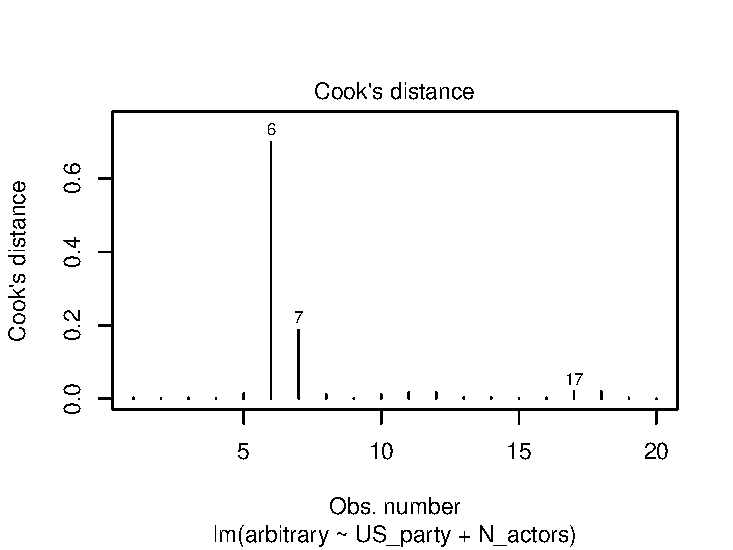
\includegraphics{messydates_article_files/figure-latex/outliers-1} \end{center}

\end{CodeChunk}

\hypertarget{conclusion}{%
\section{Conclusion}\label{conclusion}}

Dates are often messy. Researchers recognize date messiness and, thanks
to \pkg{messydates}, are no longer required to force non-existent
precision on data to proceed with analysis. \pkg{messydates} implements
for R the `mdate' class to help researchers retain and work with various
kinds of date imprecision. The class allows regular dates to be
annotated to express unspecified, approximate or uncertain date
components, date ranges, and sets of dates, according to ISO standards.
\pkg{messydates} includes functions for expanding, and contracting,
annotated sets or ranges of dates. Methods for explicitly resolving
annotated sets or range of dates into precise dates are also offered.

\hypertarget{acknowledgements}{%
\section{Acknowledgements}\label{acknowledgements}}

We would like to thank the Swiss National Science Foundation. This work
was supported by grant number 188976.

\renewcommand\refname{References}
\bibliography{references.bib}



\end{document}
